\section{问题四模型的建立与求解}

\subsection{建模思路}

问题四的微网物理结构继续沿用问题二、三，新的关键变化是：外部电网实时电价也成为未来未知量。每天0:00或日内阶段制定计划时，附件4中尚未发生的真实价格不能提前进入优化模型，只能用于历史训练、已发生时段更新、事后真实结算和模型评价。

因此：

\[
\boxed{
Q4\text{-}2
=
Q2
+
\text{电价预测}
+
\text{价格误差 SAA}
}
\]

以及

\[
\boxed{
Q4\text{-}3
=
Q3
+
\text{电价预测}
+
\text{日内价格更新}
+
\text{价格误差 SAA}
}.
\]

问题四在问题二、三已有负荷和光伏随机性的基础上进一步形成 负荷、光伏、电价 三类联合不确定量。

\subsection{电价预测与价格误差库}

设附件4已实现真实电价为 \(\pi^{act}_{d,t}\)， 计划阶段中心预测为 \(\hat\pi_{d,t}\)， SAA 中第 \(\omega\) 个价格情景为 \(\pi^{(\omega)}_{d,t}\)。 必须满足

\begin{equation}
\boxed{
\text{未来 }\pi^{act}\text{ 不得提前进入计划优化}
}.
\end{equation}

电价中心预测采用与问题二预测框架一致的“同周期回溯 + 偏差校正”。每天0:00只使用历史真实价格预测未来7日：

\begin{equation}
\hat\pi_{\tau,t}^{(d)},
\qquad
\tau=d,\ldots,d+6.
\end{equation}

定义历史价格残差

\begin{equation}
e^\pi_{r,t}
=
\pi^{act}_{r,t}
-
\hat\pi_{r,t}.
\end{equation}

每个历史日保留完整144槽价格误差向量，并使用最近28个有效残差日。

问题四中的未来随机量包括 负荷、光伏、电价。 为尽量保留三者的历史共同结构，同一个 SAA 情景中的 \(e^L\)、\(e^{PV}\)、\(e^\pi\) 尽量从同一历史日期联合抽取。

正式情景数取 \(K=4\)， 稳定性分析取 \(K=8\)， 随机种子为2026。

价格情景为 \(\pi^{(\omega)}
=
\hat\pi+e^\pi\)。 历史残差叠加后可能出现负价格，因此模型保留负价格情景，不将其人工截断为0。

\subsection{Q4-2：考虑负荷、光伏与电价联合不确定性的7日滚动模型}

每天0:00同时预测未来负荷、光伏和电价，形成联合随机情景 \(\left(
L^{(\omega)},
PV^{(\omega)},
\pi^{(\omega)}
\right)\)。 第一阶段变量继续为 \(G^{plan}_{d,t}\)， 并对所有情景保持一致。

第二阶段继续沿用问题二的物理执行变量 \(G^L,\ G^{ch},\ PV^{ch},\ C,\ D,\ E,\ V,\ W,\ H,\ u\)，
物理约束与问题二逐条相同（负荷平衡、充电来源、光伏剩余、储能递推、容量与功率上下限、
充放电互斥），只是情景由负荷与光伏两维扩展为负荷、光伏、电价三维。计划与执行的连接关系为

\begin{equation}
G^L+G^{ch}+W=G^{plan}.
\end{equation}

Q4-2的随机优化目标为

\begin{equation}
\min Z_d^{4-2}
=
\frac1K
\sum_{\omega=1}^{K}
\left[
C_d^{plan,(\omega)}
+
C_d^{em,(\omega)}
+
C_d^{future,(\omega)}
\right],
\end{equation}

其中

\begin{equation}
\begin{gathered}
C_d^{plan,(\omega)}
=
\sum_t
\pi_{d,t}^{(\omega)}
G_{d,t}^{plan}
\Delta t,\\
C_d^{em,(\omega)}
=
\sum_t5\pi_{d,t}^{(\omega)}
H_{d,t}^{(\omega)}
\Delta t.
\end{gathered}
\end{equation}

未来 continuation cost 同样使用对应的价格情景。

最终报送费用不能使用预测价格，而应使用附件4的真实实现价格：

\begin{equation}
C_d^{4-2,act}
=
\sum_t
\left[
\pi_{d,t}^{act}G_{d,t}^{plan}
+
5\pi_{d,t}^{act}H_{d,t}^{act}
\right]\Delta t.
\end{equation}

\subsection{Q4-3：加入光伏预报与价格日内更新}

Q4-3继承问题三的0:00、6:00、12:00、18:00四阶段结构。0:00：0:00时负荷采用问题二自建预测，光伏采用附件3的0:00最新预报，电价采用0:00价格预测。6:00、12:00、18:00：

三个调整时点均保持负荷中心预测为当天0:00版本，把光伏中心预测切换为当前时刻附件3的最新预报，允许电价预测利用已发生的真实价格作因果更新；同时锁定已执行时段，并以当前真实储电量作为新阶段初值。

设当天基础价格预测为 \(\hat\pi_{d,t}^{base}\)。 阶段 \(s\) 只允许使用 \(\{\pi^{act}_{d,\tau}:\tau<s\}\) 中已经发生的真实价格构造日内校正项 \(b_{d,s}\)，则剩余时段中心预测写为

\begin{equation}
\hat\pi_{d,t}^{(d,s)}
=
\hat\pi_{d,t}^{base}
+
b_{d,s},
\qquad
t\ge s.
\end{equation}

日内更新不使用未来真实价格。

四个阶段分别维护价格残差库

\[
\mathcal E_\pi^0,\quad
\mathcal E_\pi^6,\quad
\mathcal E_\pi^{12},\quad
\mathcal E_\pi^{18},
\]

定义

\begin{equation}
e^{\pi,s}_{r,\ell}
=
\pi^{act}_{r,\ell}
-
\hat\pi^{(r,s)}_{r,\ell}.
\end{equation}

阶段 \(s\) 的联合随机情景为

\[
L^{(\omega)}
=
\hat L+e^L,\\
PV^{(\omega,s)}
=
\widehat{PV}^{(s)}
+
e^{PV,s},
\]

\begin{equation}
\pi^{(\omega,s)}
=
\hat\pi^{(s)}
+
e^{\pi,s}.
\end{equation}

\subsection{Q4-3计划与调整变量}

0:00原始计划：

\[
P_{d,t}.
\]

6:00、12:00、18:00调整计划：

\[
A^6_{d,t},
\qquad
A^{12}_{d,t},
\qquad
A^{18}_{d,t}.
\]

最终生效计划为

\begin{equation}
B_{d,t}
=
\begin{cases}
P_{d,t},&0\le t<6,\\
A^6_{d,t},&6\le t<12,\\
A^{12}_{d,t},&12\le t<18,\\
A^{18}_{d,t},&18\le t<24.
\end{cases}
\end{equation}

所有调整统一相对于当天0:00原始计划结算：

\begin{equation}
A-P
=
\Delta^+-\Delta^-.
\end{equation}

与问题三不同，问题四的价格情景可能为负值，因此不能依靠正价格条件自动保证 \(\Delta^+\) 与 \(\Delta^-\) 单边取值，需要增加专门约束。

\subsection{H-1：负价格下的计划购电物理上界}

负价格情景下若计划购电没有上界，模型可能为获得负成本收益而购买大量无实际用途的电量并全部进入 \(W\)。
正常购电的实际用途只有补负荷与给储能充电，因此取当前日的计划购电物理上界为

\begin{equation}
\begin{gathered}
U_{d,t}=\max_{\omega}\overline L_{d,t}^{(\omega)}+P_{\max},
\qquad0\le P_{d,t}\le U_{d,t},\\
0\le G_{\tau,t}^{plan,(\omega)}\le\overline L_{\tau,t}^{(\omega)}+5000,
\end{gathered}
\end{equation}

即最多补足最大情景的负荷缺口并按最大功率充电。这样 \(W\) 只表示预测误差造成的已购未用电，
不能成为负价格套利通道。

\subsection{H-2：调增与调减显式互斥}

负价格条件下，只设置 \(A-P=\Delta^+-\Delta^-\) 与 \(\Delta^+,\Delta^-\ge0\) 可能出现两者同时为正的非业务解，
故增加二元变量 \(z_t\) 使调增与调减互斥：

\begin{equation}
0\le\Delta_t^+\le M_tz_t,
\qquad0\le\Delta_t^-\le M_t(1-z_t),
\qquad
z_t\in\{0,1\},
\qquad
M_t=U_{d,t},
\end{equation}

其中 Big-\(M\) 不使用人工大数而取上一小节给出的物理上界 \(U_{d,t}\)，
从而严格实现 \(\Delta^+=\max(A-P,0)\) 与 \(\Delta^-=\max(P-A,0)\)。

\subsection{Q4-3费用与目标函数}

阶段 \(s\) 的优化价格采用情景价格 \(\pi^{(\omega,s)}\)，时段调整按1.5倍与0.5倍结算，
紧急购电按5倍结算，因此0:00与各调整阶段的目标函数统一写为

\begin{equation}
\begin{gathered}
\min Z_{d,s}^{4-3}=\frac1K\sum_\omega\left[C^{settle,s,(\omega)}+C^{em,s,(\omega)}+C^{future,s,(\omega)}\right],\\
C^{settle,s,(\omega)}=\left[\pi^{(\omega,s)}P+1.5\pi^{(\omega,s)}\Delta^+-0.5\pi^{(\omega,s)}\Delta^-\right]\Delta t,
\end{gathered}
\end{equation}

其中0:00阶段的结算基准为原始计划 \(P\)，调整阶段为各阶段的调整计划。
最终报送时全部替换为真实电价 \(\pi^{act}\)：

\begin{equation}
\begin{gathered}
C_d^{4-3,act}=C_d^{normal,act}+C_d^{em,act},\\
C_d^{normal,act}=\sum_t\left[\pi^{act}_{d,t}P_{d,t}+1.5\pi^{act}_{d,t}\Delta^+_{d,t}-0.5\pi^{act}_{d,t}\Delta^-_{d,t}\right]\Delta t,\\
C_d^{em,act}=\sum_t5\pi^{act}_{d,t}H^{act}_{d,t}\Delta t.
\end{gathered}
\end{equation}

\subsection{模型求解}

Q4-2经联合情景展开后属于7日滚动两阶段 SAA-MILP，Q4-3属于日内多阶段滚动 SAA-MILP。 两者的连续能量流变量与二元充放电状态、Q4-3的调增调减互斥状态共同构成混合整数线性规划。

底层继续采用分支定界/分支切割，并利用 MATLAB \texttt{intlinprog} 求解。首先求解 LP 松弛作为热启动，再对非整数变量进行分支，通过节点下界、整数上界和切平面逐步缩小搜索空间。

Q4-2每天把负荷预测、光伏预测与电价预测联合抽样为 SAA 情景，经7日滚动 MILP 输出当天计划，再按真实数据执行并更新储电量。

Q4-3的日内执行方式为：0:00用负荷预测、光伏预报与价格预测求原始计划 \(P\)；执行至6:00后读取新的光伏预报、已实现价格与真实储电量，求调整计划 \(A^6\)；此后按同样方式在12:00与18:00分别求 \(A^{12}\) 与 \(A^{18}\)，并执行至24:00。
即坚持“求解、执行、更新真实状态与价格信息、再求解”的循环。

\subsection{结果分析框架}

\begin{table}[H]
\centering
\zihao{5}
\begin{tabular}{lrrrr}
\toprule
指标 & Q2固定电价 & Q4-2波动电价 & Q3固定电价 & Q4-3波动电价 \\
\midrule
总费用/元 & 14806890.28 & 16320514.83 & 14485230.30 & 15225713.07 \\
正常+调整费用/元 & — & 13737348.89 & 13451415.12 & 14148292.42 \\
紧急购电费用/元 & 1657825.30 & 2583165.94 & 1033815.18 & 1077420.65 \\
紧急购电量/kWh & 269240.94 & 450371.13 & 185523.91 & 200511.20 \\
已购未用电/kWh & 1136190.28 & 1061902.30 & 601472.99 & 566918.30 \\
日末储电量均值/kWh & 7045.97 & 4810.16 & 6847.95 & 4831.70 \\
\bottomrule
\end{tabular}
\caption{问题四两口径费用与紧急购电对照（费用单位：元，电量单位：kWh）}
\label{tab:11}
\end{table}

结果分析应重点回答：

结果分析围绕六个问题展开：波动价格相对于固定价格如何改变总成本；储能是否表现出更明显的低价充电、高价放电；电价预测误差造成多少额外成本；Q4-3的日内光伏与价格更新是否进一步降低紧急购电或调整成本；负价格情景下 H-1/H-2是否被实际激活；以及价格峰谷预测偏差如何影响储能调度时机。

\subsection{电价预测与价格风险检验}

电价预测精度使用

\[
MAE_\pi
=
\frac1N
\sum_i
|\hat\pi_i-\pi_i^{act}|,
\]

\begin{equation}
RMSE_\pi
=
\sqrt{
\frac1N
\sum_i
(\hat\pi_i-\pi_i^{act})^2
}.
\end{equation}

中心预测与实测电价的逐时段对照（取2025年7月14日至7月20日）见图~\ref{fig:q4-week}。

\begin{figure}[htbp]
\centering
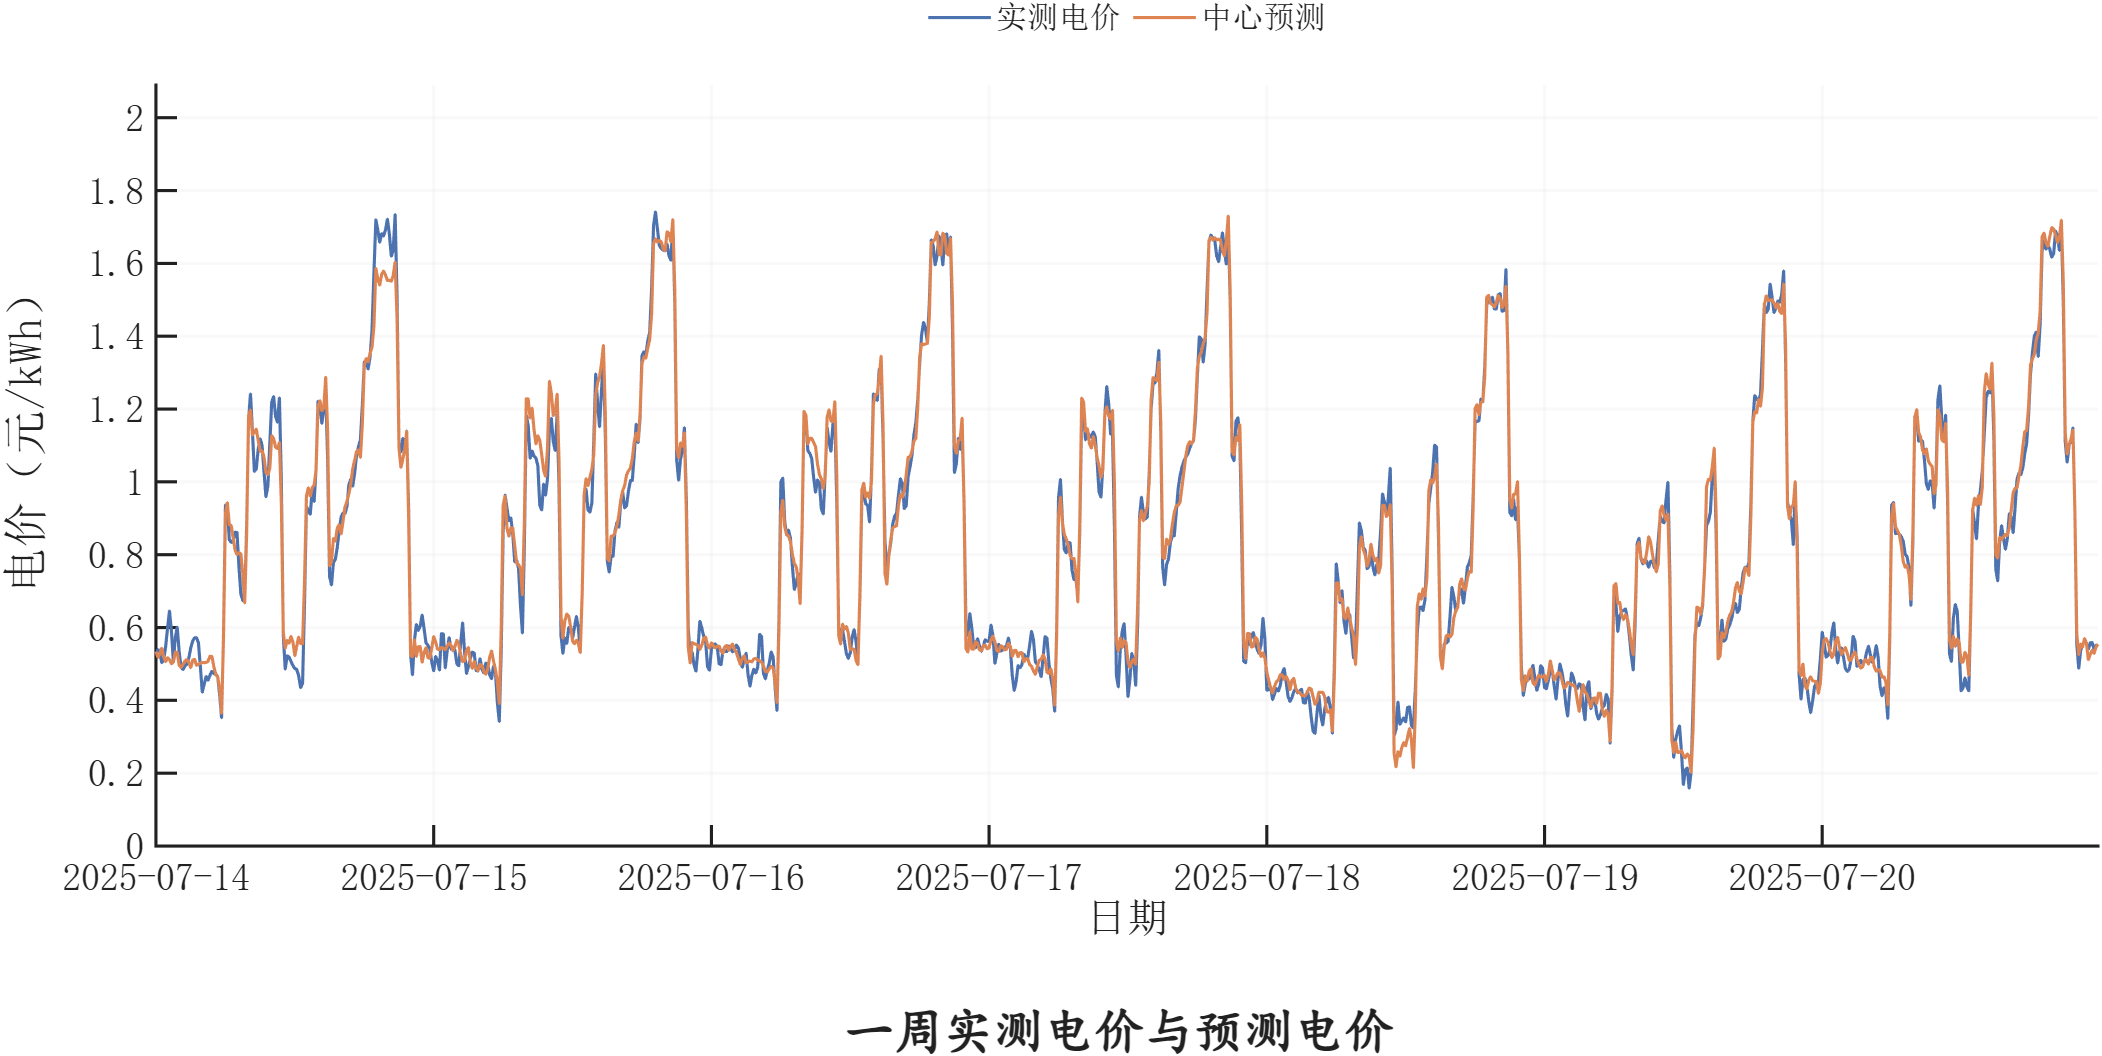
\includegraphics[width=0.78\textwidth,height=0.26\textheight,keepaspectratio]{figures/q4_price_week.png}
\caption{一周中心电价预测与实测电价对照（电价单位：元/kWh）}
\label{fig:q4-week}
\end{figure}

中心预测能够刻画日内峰谷形态，高低价时段基本对齐，该周预测对实测的 MAE 为0.0371元/kWh；但峰谷出现的具体时刻仍有偏差。

\begin{table}[H]
\centering
\zihao{5}
\begin{tabular}{lr}
\toprule
指标 & 数值 \\
\midrule
MAE & 0.0432 \\
RMSE & 0.0602 \\
峰值时刻精确命中率 & 36.2\% \\
谷值时刻精确命中率 & 33.8\% \\
峰值1h 内命中率 & 63.5\% \\
谷值1h 内命中率 & 58.4\% \\
峰谷差预测 MAE & 0.0675 \\
\bottomrule
\end{tabular}
\caption{电价预测精度指标（误差单位：元/kWh）}
\label{tab:12}
\end{table}

同时以只按中心价格预测的方案 \(P0\) 与含价格误差 SAA 的方案 \(P1\) 作消融对比，衡量价格风险建模的贡献。

建立“未来真实价格提前已知”的完美价格信息基准，用于计算价格不确定性代价：

\begin{equation}

\Delta C_{\rm price}
=
C_{\rm forecast}
-
C_{\rm perfect-price}.
\end{equation}

电价预测的逐小时误差画像见图~\ref{fig:q4-prof}。

\begin{figure}[htbp]
\centering
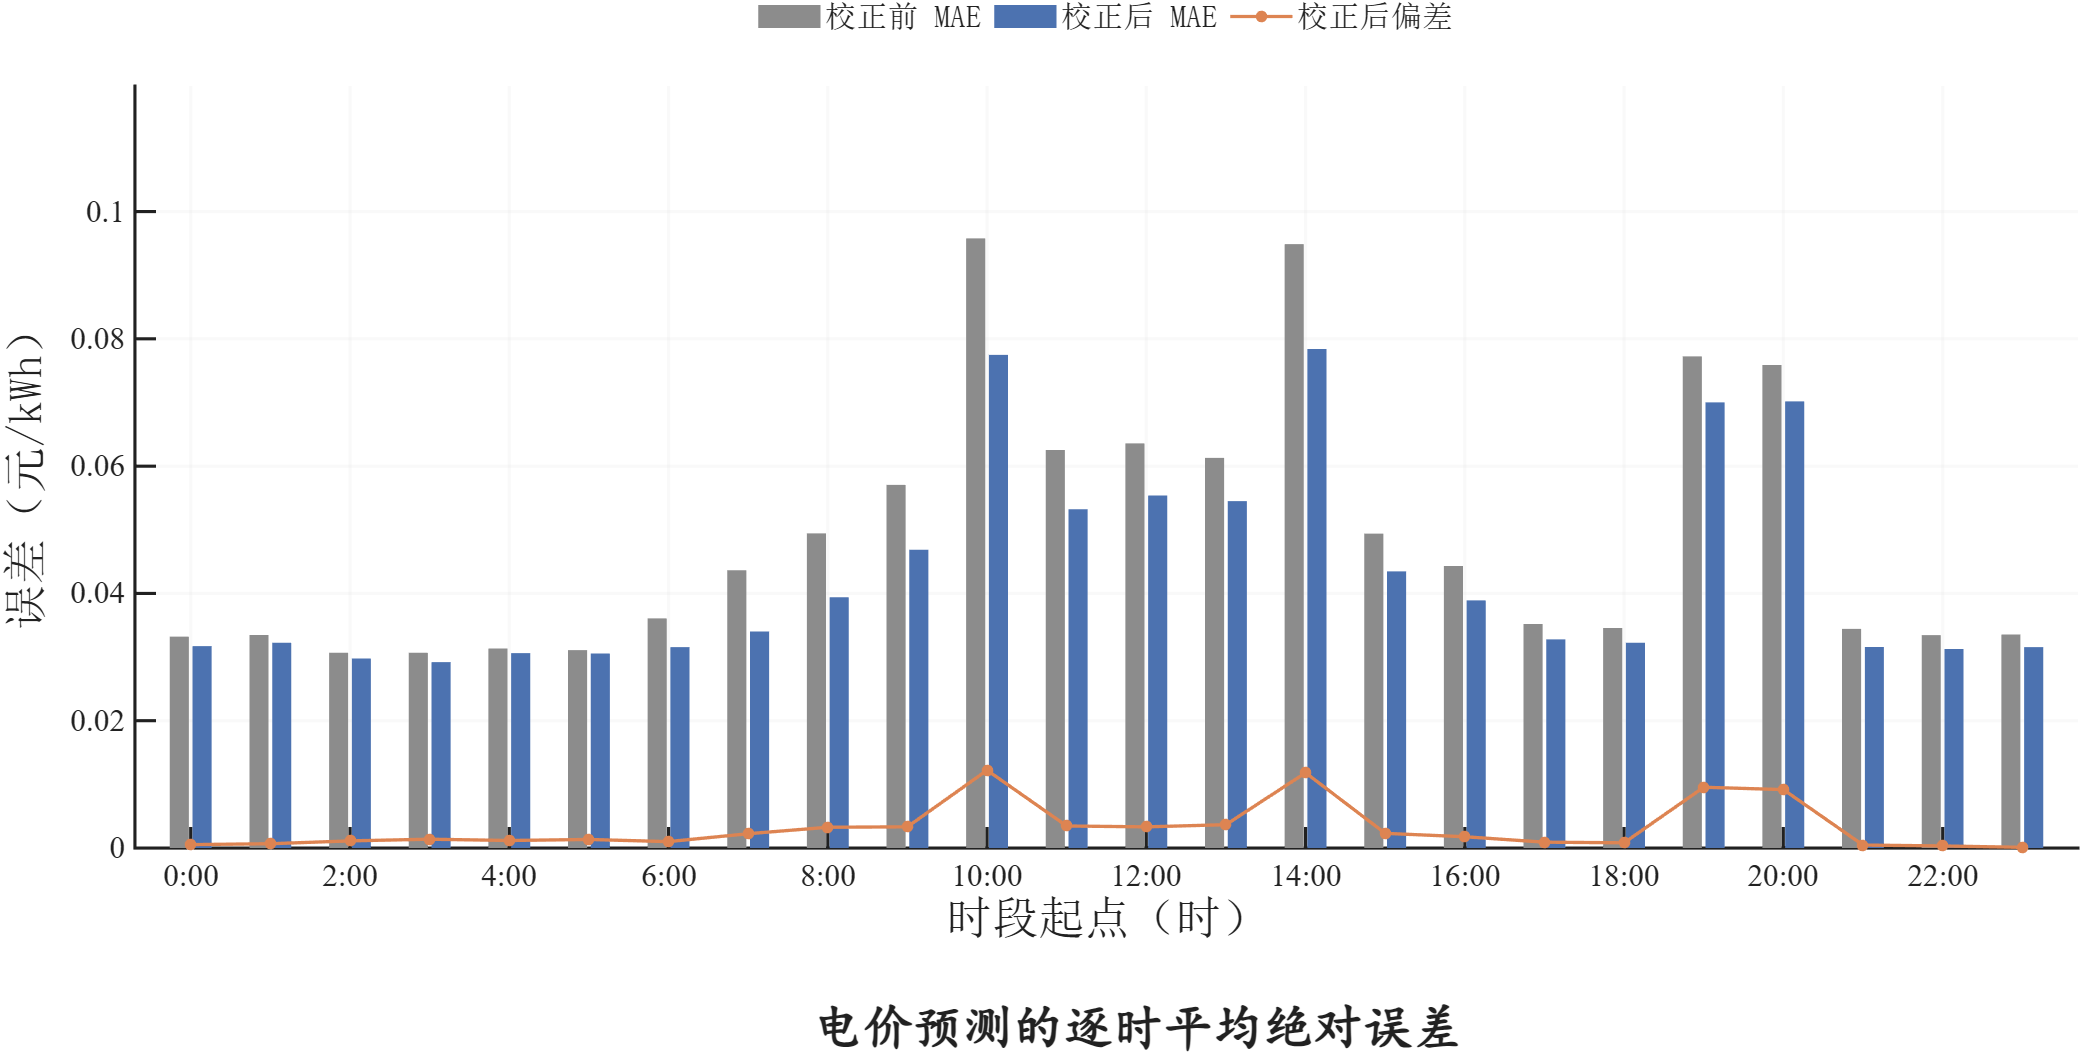
\includegraphics[width=0.78\textwidth,height=0.26\textheight,keepaspectratio]{figures/q4_price_profile.png}
\caption{电价预测的逐小时误差画像（误差单位：元/kWh）}
\label{fig:q4-prof}
\end{figure}

经逐小时偏差校正后各小时误差普遍下降，整体 MAE 由0.0489降至0.0432元/kWh，改善11.57\%，校正后残余偏差最大仅0.0122元/kWh。误差的时段分布并不均匀，清晨与傍晚相对更大，逐时 MAE 的最大值出现在10:00—11:00。

其结果为\(
\Delta C_{\rm price}
=
\text{66993.37元}.
\)

\subsection{模型检验}

问题四除继续检查能量平衡、储能递推、充放电互斥、正常购电守恒和非预见性外，还应检查：

校验覆盖未来真实价格无泄漏、三类误差同日联合抽样、Q4-3阶段价格更新的因果性、最终费用按真实价格重算，以及紧急购电按 \(5\pi^{act}\)、调增调减按 \(1.5\pi^{act}\) 与 \(0.5\pi^{act}\) 结算；同时确认 H-1计划购电物理上界与 H-2调增调减互斥均生效，负价格情景不导致模型无界、\(W\) 不出现负价套利，阶段执行与最终重放一致。

H-2启用后，应有 \(\#\{t:\Delta_t^+>0\text{ 且 }\Delta_t^->0\}=0\)。 最大等式残差：\(6.96\times10^{-10}.\)最大整数间隙：
\(1.16\times10^{-3}.\)最大拼接重放偏差：\(0.\)

稳定性分析比较 \(K=4\) 与 \(K=8\)：

\begin{table}[H]
\centering
\zihao{5}
\begin{tabular}{lrrr}
\toprule
指标 & \(K=4\) & \(K=8\) & 相对差异 \\
\midrule
Q4-2总费用 & 16320514.83 & 16240197.29 & $-0.49\%$ \\
Q4-3总费用 & 15225713.07 & 15100131.61 & $-0.82\%$ \\
Q4-2紧急购电量 & 450371.13 & 441055.51 & $-2.07\%$ \\
Q4-3紧急购电量 & 200511.20 & 186767.09 & $-6.85\%$ \\
\bottomrule
\end{tabular}
\caption{问题四 Q4-2与 Q4-3指标对照}
\label{tab:13}
\end{table}
